\documentclass[submit]{harvardml}

\course{CS181-S20}
\assignment{Assignment \#2}
\duedate{11:59pm Feb 21st, 2020}

\usepackage[OT1]{fontenc}
\usepackage[colorlinks,citecolor=blue,urlcolor=blue]{hyperref}
\usepackage[pdftex]{graphicx}
\usepackage{subfig}
\usepackage{fullpage}
\usepackage{amsmath}
\usepackage{amssymb}
\usepackage{color}
\usepackage{soul}
\usepackage{todonotes}
\usepackage{listings}
\usepackage{common}
\usepackage{enumitem}
\usepackage{bm}
\newcommand{\B}{\text{B}}
\newcommand{\Beta}{\text{Beta}}

\usepackage[mmddyyyy,hhmmss]{datetime}

\definecolor{verbgray}{gray}{0.9}

\lstnewenvironment{csv}{%
  \lstset{backgroundcolor=\color{verbgray},
  frame=single,
  framerule=0pt,
  basicstyle=\ttfamily,
  columns=fullflexible}}{}

\begin{document}

\begin{center}
{\Large Homework 2: Classification and Bias-Variance Trade-offs}\\
\end{center}

\subsection*{Introduction}

This homework is about classification and bias-variance trade-offs. In
lecture we have primarily focused on binary classifiers trained to
discriminate between two classes. In multiclass classification, we
discriminate between three or more classes. We encourage you
to read CS181 Textbook's Chapter 3 for more information on linear
classification, gradient descent, classification in the discriminative
setting (covers multiclass logistic regression and softmax), and
classification in the generative setting. Read Chapter 2.8 for more
information on the trade-offs between bias and variance.

As a general note, for classification problems we imagine that we have the input matrix $\boldX \in
\reals^{n \times m}$ (or perhaps they have been mapped to some basis
$\bm{\Phi}$, without loss of generality) with outputs now
"one-hot encoded."  This means that if there are~$c$ output
classes, rather than representing the output label $y$ as an
integer~${1,2,\ldots,c}$, we represent $\boldy$ as a "one-hot" vector of
length~$c$. A "one-hot" vector is defined as having every component equal to 0 except for 
a single component which has value equal to 1.
For example, if there are $c = 7$ classes and a particular data point belongs to class 3, 
then the target vector for this data point would be~$\boldy = [0,0,1,0,0,0,0]$.
We will define $C_1$ to be the one-hot vector for the 1st class, $C_2$ for the 2nd class, etc.
Thus, in the previous example $\boldy = C_3$. If there are $c$ total classes, then the set of
possible labels is $\{C_1 \ldots C_c \} = \{C_k\}_{k=1}^c$.
Throughout the assignment we will assume
that each label $\boldy \in \{C_k\}_{k=1}^c$.\\

In problems 1 and 3, you may use \texttt{numpy} or
\texttt{scipy}, but not \texttt{scipy.optimize} or \texttt{sklearn}. Example code given is in Python 3. \\

Please type your solutions after the corresponding problems using this
\LaTeX\ template, and start each problem on a new page.\\

Please submit the \textbf{writeup PDF to the Gradescope assignment `HW2'}. Remember to assign pages for each question. \\

Please submit your \textbf{\LaTeX\ file and code files to the Gradescope assignment `HW2 - Supplemental'}. 

You can use a \textbf{maximum of 2 late days} on this assignment.  Late days will be counted based on the latest of the two submissions. \\

%%%%%%%%%%%%%%%%%%%%%%%%%%%%%%%%%%%%%%%%%%%%%
% Problem 1
%%%%%%%%%%%%%%%%%%%%%%%%%%%%%%%%%%%%%%%%%%%%%
\begin{problem}[Exploring Bias and Variance, 10 pts]
  In this problem, we will explore the bias and variance of a couple
  of different model classes when it comes to classification.

  The data have one-dimensional inputs $x$ and binary outputs $y$.
  
\begin{csv}
x, y
-8, 1
-3, 0
-2, 1
-1, 0
0, 0
1, 0
2, 1
3, 1
4, 1
5, 1
\end{csv} 

\begin{enumerate}

\item Fit a linear classifier based off the value of sigmoid($w^T \phi$)
 (using a decision threshold of 0.5) with the bases $\phi_1(x) = [1, x]$,
  $\phi_2(x) = [1, x, x^2]$, $\phi_3(x) = [1, x, x^2, x^3, x^4, x^5, x^6]$ and
  a logistic loss with gradient descent. Note that the classes are represented
  with 0's and 1's. 
  Repeat your gradient descent 25 times for each basis option, with different
   random starting values of $w$. Use $\eta=0.001$ and take 10000 steps
   for each run, and make sure to average the gradient over the data points
   (for each step). These parameters, while not perfect, will ensure your code
   runs in a reasonable amount of time. The emphasis of this problem is on
   capturing the bias-variance trend, so don't worry the exact details of the
   models as long as this trend is captured. Hint: if you run into $\log(0)$ issues
   in the logistic loss function, you can use a small $\epsilon=0.000001$ to take care of it.


\item Create three plots, one for each basis. On each plot, first plot the
  the data points as given above, then plot the prediction functions
  of the top 10 runs (in terms of loss) of gradient descent. Explicitly, 
  the prediction function of a given model is essentially plotting sigmoid($w^T \phi(x)) > 0.5$
  for all x's (seen in the starter code with a random w that you will need to change).
  While unlikely, in case all 25 runs were poor, you may need to rerun your code.
    
\item Explain what you see in terms of the bias-variance trade-off.

\item If we were to have "triple" the data, as in add in (-6.33, 1), (-4.67, 0), (-2.67, 0), (-2.33, 1) ... (4.33, 1), (4.66, 1), how would the variance change (no need to rerun your code, just answer this 
  as a conceptual question)? Why do you think that may be the case? See graph below for reference. \\
  
\underline{If we had triple the data:} \\

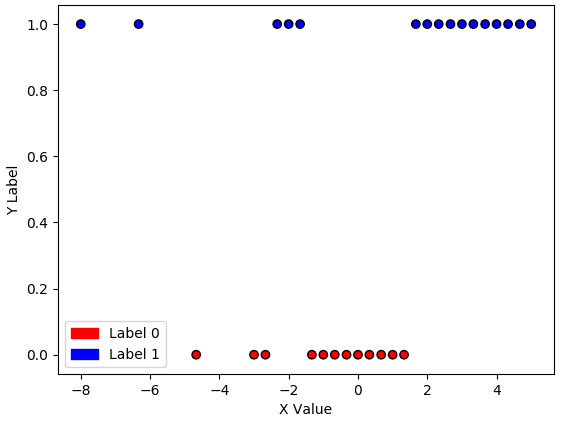
\includegraphics[scale=0.45]{tripleddata.png}
  
\end{enumerate}

\end{problem}

\newpage

\subsection*{Solution}

%%%%%%%%%%%%%%%%%%%%%%%%%%%%%%%%%%%%%%%%%%%%%
% Problem 2
%%%%%%%%%%%%%%%%%%%%%%%%%%%%%%%%%%%%%%%%%%%%%
\begin{problem}[Matrix calculus, 15pts]

  Consider now a generative $c$-class model.  We adopt class prior
  $p(\boldy = C_k; \bpi) = \pi_k$ for all $k \in \{1, \ldots, c\}$
(where $\pi_k$ is a parameter of the prior).
Let  $p(\boldx|\boldy=C_k)$ denote
the class-conditional density of features $\boldx$ (in this
case for class $C_k$). Consider the data set $D = \{(\boldx_i,
\boldy_i)\}_{i=1}^n$ where as above $\boldy_i \in \{C_k\}_{k=1}^c$ is
encoded as a one-hot target vector and the data are independent.

\begin{enumerate}
  \item Write out the negative log-likelihood of the data set, $-\ln p(D ; \bpi)$.

  \item Since the prior forms a distribution, it has the constraint that
    $\sum_k\pi_k - 1 = 0$.  Using the hint on
Lagrange multipliers below, give the
    expression for the maximum-likelihood estimator for the prior
    class-membership probabilities, i.e.
    $\hat \pi_k.$
    Make sure to write out the intermediary equation you need
    to solve to obtain this estimator. Double-check your answer: the final
    result should be very intuitive!
\end{enumerate}

    For the remaining questions, let the
    class-conditional probabilities be Gaussian distributions with
the same covariance matrix
    $$p(\boldx | \boldy = C_k) = \mathcal{N}(\boldx |  \bmu_k, \bSigma), \text{\ for\ }k \in \{1,\ldots, c\}$$ 
    and different means $\bmu_k$ for each class.

    \begin{enumerate}
  \item[3.] Derive the gradient of the negative log-likelihood with respect to vector $\bmu_k$.
    Write the expression in matrix form as a function of the variables defined
    throughout this exercise. Simplify as much as possible for full credit.
  \item[4.] Derive the maximum-likelihood estimator $\hat{\mu}_k$ for vector $\bmu_k$. Once
    again, your final answer should seem intuitive.
  \item[5.] Derive the gradient for the negative log-likelihood with respect to the
    covariance matrix $\bSigma$ (i.e., looking
to find an MLE for the covariance).
Since you are differentiating with respect to a
    \emph{matrix}, the resulting expression should be a matrix!
%
  \item[6.] Derive the maximum likelihood estimator $\hat{\Sigma}$ of the covariance matrix.
\end{enumerate}

\paragraph{Hint: Lagrange Multipliers.} Lagrange Multipliers are a method for
optimizing a function $f$ with respect to an
equality constraint, i.e.
\[\min_{\boldx} f(\boldx)\ \text{s.t.}\ g(\boldx) = 0.\]

This can be turned into an unconstrained problem by introducing a
Lagrange multiplier $\lambda$ and constructing the Lagrangian function,
\[L(\boldx, \lambda) =  f(\boldx) + \lambda g(\boldx).\]

It can be shown that it is a necessary condition that the optimum
is a critical point of this new function. We can find this point by solving two equations:

\[\frac{\partial L(\boldx, \lambda)}{\partial  \boldx} = 0  \ \ \text{and}\  \  \frac{\partial L(\boldx, \lambda)}{\partial \lambda} = 0 \]


\paragraph{Cookbook formulas.} Here are some formulas you might want to consider
using to compute difficult gradients. You can use them  in the homework
without proof. If you are looking to hone your matrix calculus skills, try to
find different ways to prove these formulas yourself (will not be part of the
evaluation of this homework). In general, you can use any formula from the matrix cookbook,
as long as you cite it. We opt for the following common notation:
$\boldX^{-\top} := (\boldX^{\top})^{-1}$
\begin{align*}
  & \frac{\partial \bolda^\top \boldX^{-1} \boldb}{\partial \boldX} = - \boldX^{-\top} \bolda \boldb^\top \boldX^{-\top} \\
  & \frac{\partial \ln | \det (\boldX) |}{\partial \boldX} = \boldX^{-\top}
 \end{align*}
 \end{problem}


\subsection*{Solution}

%%%%%%%%%%%%%%%%%%%%%%%%%%%%%%%%%%%%%%%%%%%%%
% Problem 3
%%%%%%%%%%%%%%%%%%%%%%%%%%%%%%%%%%%%%%%%%%%%%

\begin{problem}[Classifying Stars, 15pts]

You're tasked with classifying three different kinds of stars, based
on their magnitudes and temperatures. See star.png for a plot of
the data, adapted from
\url{http://astrosci.scimuze.com/stellar_data.htm} and available as
\verb|data/hr.csv|, which you will find in the Github repository. \\

The CSV file has three columns: type, magnitude, and temperature. The
first few lines look like this:
\begin{csv}
Type,Magnitude,Temperature
Dwarf,-5.8,-0.35
Dwarf,-4.1,-0.31
...
\end{csv}

In this problem, you will code up 4 different classifiers for this task:
\begin{enumerate}[label=\alph*)]
\item \textbf{A three-class generalization of logistic regression}, also
  known as softmax regression. You will do this by
  implementing gradient descent on the negative log-likelihood. You
  will need to find good values for the learning rate $\eta$ (\texttt{self.eta}) and
  regularization strength $\lambda$ (\texttt{self.lam}). Make sure to include a bias term and to
  use L2 regularization. See CS181 Textbook's Chapter 3.6 for more details on multi-class
  logistic regression and softmax.
  
\item \textbf{A generative classifier with Gaussian class-conditional
  densities with a \textit{shared covariance} matrix} across all classes. 
  Feel free to re-use your Problem 2 results.
\item \textbf{Another generative classifier with Gaussian class-conditional densities , but now 
with a \textit{separate covariance} matrix} learned for each class. (Note: 
The staff implementation can switch between the two Gaussian generative classifiers with just a
few lines of code.)

\item \textbf{A kNN classifier} in which you classify based on the $k=1,3,5$ nearest neighbors and the following distance function: dist(star$_1$, star$_2$) = ((mag$_1$ - mag$_2)/3)^2$ + (temp$_1$ - temp$_2)^2$ (where nearest neighbors are those with the smallest distances from a given point). 

Note: because we are predicting over a continuous space (not just the training data), we omit the step of making each training point ignore itself when selecting neighbors).

\end{enumerate}

After implementing the above classifiers, complete the following exercises:

\begin{enumerate}
    \item Plot the decision boundaries generated by each classifier for the dataset. Include them in your PDF. 
    Identify the similarities and differences among the classifiers. What explains the differences?
    
    \item For logistic regression only, make a plot with
      "Number of Iterations" on the x-axis and "Negative Log-Likelihood Loss" on the y-axis for several
      configurations of hyperparameters. Note which configuration yields
      the best final loss. What are your final choices of learning rate
      ($\eta$) and regularization strength ($\lambda$), and why are they reasonable? How
      does altering these hyperparameters affect the ability to converge and the rate of convergence (a
      qualitative description is sufficient)?

    \item For both Gaussian generative models, report the negative log-likelihood loss. Which model has a lower loss, and why?
      For the separate covariance model, be sure to use
      the covariance matrix that matches the true class of each data
      point.
    
    \item Consider a star with Magnitude 6 and Temperature 2.
      To what class does each classifier assign this star? Do the
      classifiers give any indication as to whether or not you should
  trust them?
\end{enumerate}

\textbf{Implementation notes:} Run the controller file, \texttt{T2\_P3.py},
to test your code. Write the actual implementations in the \texttt{GaussianGenerativeModel},
\texttt{LogisticRegression}, and \texttt{KNNModel} classes, which are defined in the three
\texttt{T2\_P3\_ModelName.py} files. These classes follow the same interface pattern
as sklearn. Their code
currently outputs nonsense predictions just to show the
high-level interface, so you should replace their \texttt{predict()} implementations.
You'll also need to modify the hyperparameter
values in \texttt{T2\_P3.py} for logistic regression.

\end{problem}



\subsection*{Solution}

\newpage
%%%%%%%%%%%%%%%%%%%%%%%%%%%%%%%%%%%%%%%%%%%%%
% Name and Calibration
%%%%%%%%%%%%%%%%%%%%%%%%%%%%%%%%%%%%%%%%%%%%%
\subsection*{Name}

\subsection*{Collaborators and Resources}
Whom did you work with, and did you use any resources beyond cs181-textbook and your notes?

\subsection*{Calibration}
Approximately how long did this homework take you to complete (in hours)? 



\end{document}
